\chapter{Introduction to Assembly - A Bottom Up Approach}

One of the core principles of our Information Security and Privacy class is to focus on the fundamentals. The belief is that when we are able to understand the fundamentals and the intuition behind the most basic building blocks of security, we will be better prepared to understand new concepts when we get exposed to them. We will continue this methodology in this short tutorial on x86 assembly. 

Think back to your undergraduate studies (if you didn’t have a CS or CompE background then go and take a look at some program course schedules) and you will notice that one of the first classes you take is Digital Logic. There is a reason for this. 

Most of us are familiar with high level programming languages such as Python and C (yes I am aware that some people don’t consider C a high level language, but we will soon see that it is indeed quite high). However, some of us might not be able to trace the programs written in such languages all the way down to the most basic building blocks. 

Let’s take C for example, when we write a C program, we will normally compile the source into an object file and then link it with other objects into a single executable. The executable will undoubtedly be expressed as machine level instructions which can be immediately disassembled into an Assembly Language if desired. 

It is then up to the CPU (Central Processor Unit) to interpret the machine instructions and actually execute them. At the core of any CPU should be an Arithmetic Logic Unit (ALU) which is the main component in charge of executing many of the popular instructions. More advanced instructions might involve co-processors, but let’s just focus on the ALU at the moment.

\section{Arithmetic Logic Unit}

As the name implies, the ALU focuses on the ability to perform Arithmetic (add, subtract, etc.) and Logic (and, or, etc.) operations. But then what makes up an ALU? If we decomposed it even more, we will arrive at the basic components from digital logic. Beyond that are transistors or other means of building logic gates, which are beyond the current discussion.

So what did you learn from Digital Logic? You should have learned two types of components: discrete and sequential. Discrete logic are logic gates where the output is fully determined by the input almost instantaneously (there is always a delay). NAND gates\footnote{Remember that NAND gates can be used to construct all other logic gates}, AND gates, OR gates, XOR gates, etc. are all examples of discrete logic gates. Sequential logic gates are ones where the output depends on both the input and some notion of history. Normally this notion of history is encoded as a clock ({\tt clk}) input where the output is not determined until the {\tt clk} signal is switched on a ``rising edge'' or a ``falling edge''. The trigger doesn’t matter as much as the fact that sequential gates can remember things. This ability to remember things is why sequential logic is used to build registers which can be thought of as super fast memories.

\subsection{Building Up from Basic Gates}

Thus, given our knowledge of digital logic, we know that we have the very basic gates such as AND and OR, as well as registers due to the availability of sequential elements. Let’s focus on the AND and OR gates. 

The first question that we will want to ask is what can we do with AND and OR gates? Can we use it to create an ALU? Well given that a NAND (or NOR) gate can be used to build all other basic logic gates (\url{https://en.wikipedia.org/wiki/NAND_logic}) we know that the ``Logic'' part of ALU is covered\footnote{Not exactly since the ``shift'' is also considered a Logic operation. Shifting either left or right can be implemented using sequential elements though. Think of a ``shift register.''}  What about the ``Arithmetic'' part of the ALU? 

Well perhaps we remember that a full adder can be built using just the basic logical elements as well (\url{https://en.wikipedia.org/wiki/Adder_(electronics)#Full_adder}) meaning we have addition covered. Since subtraction is just addition with the negative of the second operand, we should have that covered as well.

But then what about multiplication?

Multiplication is a bit tricky because it is not as straightforward as the other operations. In particular, we can’t perform multiplication in a single clock tick. In other words, we can’t just build a multiplier straight out of discrete components where the output (product) will be known immediately after the inputs (multiplicands) are set. Multiplication requires some memory. Think about long multiplication such as follows:

\begin{code}
          123
x         321
----------------
          123   <--
         246    <--   Memory / Temporary Storage
        369     <--
----------------
        39483
\end{code}

Notice how we had to store the temporary products (123, 2460 and 36900) somewhere before we can add them all up to get the final product. Juxtapose this with addition where a temporary sum isn’t needed. 

At first glance there seems to be a catch-22. You need to calculate the partial products first prior to summing them up, but what about the partial products? Albeit the partial products are of a large multi-digit number with a single digit number, we still have to do multiplication. 

Luckily, we are dealing with binary numbers and binary multiplication is significantly easier to implement. The partial products are effectively multiplying the first binary number with either a 0 or a 1 meaning we can implement the partial products using AND operations.  This along with SHIFTLEFT and ADD will give us a simple multiplier (\url{https://en.wikipedia.org/wiki/Binary_multiplier}). 

Let’s look at the problem a little bit deeper. How can we get temporary memory?

\subsection{Registers for Temporary Storage}

Some of you might have observed that we can get temporary memory by creating another register. But what is a register? Why do we need it? Think about the ALU operations we have talked about thus far. They had to operate on some input, but where does this input come from and where does the output go?

Registers are fairly straightforward to explain since you have undoubtedly built them as part of your Digital Logic training. A bank of D-Flip-Flops will give you a register for example. 

Due to the fact that the operations are built using discrete components where the output is determined right when the inputs are set, we need a way to hold the inputs and outputs for a period of time so we can 1) set the inputs, 2) perform the operation and 3) read the output. 

If we didn’t apply step 1 by setting and holding (the digital logic term is latch) the input value, then the output will fluctuate along with any fluctuations in the input. Since we like stability, we would like to hold the input for a while until the output has stabilized and we have read the output. 

With regards to the output, if we didn’t perform step number 3 and read the output at the right time, we might be reading the wrong result. We ensure this by reading the output in the next clock cycle where a clock cycle is designed to be long enough for all values to settle\footnote{This delay between inputs and outputs is known as the {\em propagation delay} and is the real reason why we don't do multiplication using a big mass of discrete components. A multiplication circuit will have a long delay}.

This is why we say that these operations take 1 clock cycle by the way. We set and hold the input at clock cycle t and the discrete logic automatically gets updated to the correct output. After allowing the output to settle for one clock cycle we can then read the output at clock cycle {\em t+1}. 

In summary, the inputs and outputs are stored in registers which are subsequently built using flip-flops, the sequential elements you learned from Digital Logic. 

At this point in the tutorial, we have seen how he basic logical elements we learned from Digital Logic can be used to build the many operations that might be part of a basic ALU. This does not look like assembly though. What are we missing?

If we think of assembly, we might think of instructions - that is some way of telling the ALU which operation to perform. This is the next topic of discussion.

\section{Machine Instructions}

Right now we know that we can build the basic ALU operations, but which operation should we perform at any given time? The easiest thing for us to do is to perform all of the ALU operations at once and then let the user decide which answer they want. This is, in a way, what we do when we design complex digital circuits right? 

For example, if we want to implement the multiplier discussed previously, we might simply replicate the ALU {\em 3n} times where n is the size of the input operand in bits. We use the \inlinedcode{AND} operation in the first {\em n} ALU implementations to calculate the n partial products (one per bit). We will then use the \inlinedcode{SHIFTLEFT} operation in the next {\em n} ALU implementations to shift the partial products the number of times necessary so they are in the right location. We will then need to use the last {\em n} ALU implementations to incrementally \inlinedcode{ADD} up a shifted partial product with the temporary sum until all partial products have been summed up to obtain the final product\footnote{Note that the shifts and summation require operand sizes of {\em 2n} instead of just {\em n}}.


This is certainly feasible, but is not a very elegant design since most of these ALU implementations will be doing useless work when the multiply operation is not used. An astute student might have also recognized that if we can chain ALUs together like this, it would also means that we should be able to build a multiplier using only discrete components without the need for memory. While this is indeed true, the depth of the components will negatively affect how fast a single clock cycle can be, which means while feasible, it might not be a good idea.

What is an alternative?

In the interest of being frugal and efficient, an alternative method is to have only one single ALU that can run as fast as reasonable but then have a way to control what the ALU does during each execution and then chain the executions. In digital logic terms, this is just a multiplexer. 

\subsection{Selecting Instructions and Chaining Them}

Pictorially the idea looks something like in figure \ref{fig:IntroToAssembly:SimpleALU}. As we can see, the new reusable ALU now has three inputs, the ``Op Select'' to select the operation to use, the two operands ``Input 1'' and ``Input 2'' as well as the single output ``Output''. 

\begin{figure}
\centering
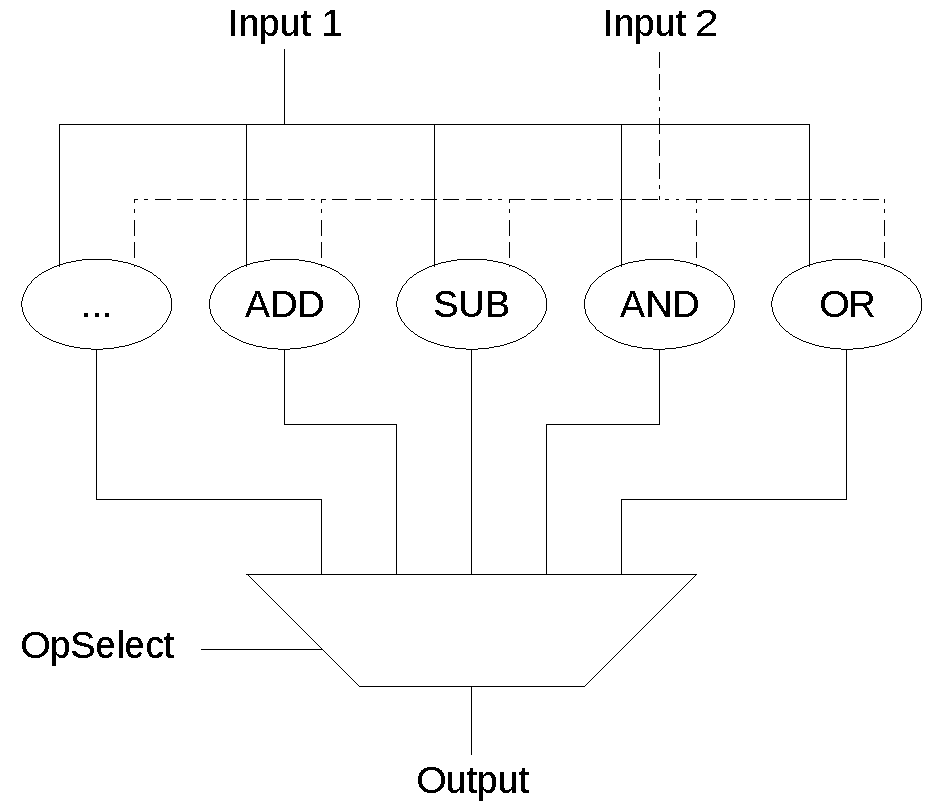
\includegraphics[width=5in]{IntroToAssembly/images/SimpleALU}
\label{fig:IntroToAssembly:SimpleALU}
\caption{A Simple ALU}
\end{figure}



While we now have the ability to select the operation to perform, we don’t yet have the ability to actually select the Inputs and Outputs. That is, in the multiplication example, we wanted to perform a sequence of binary multiplications (\inlinedcode{AND} operation), store the results in temporary locations and then perform the \inlinedcode{SHIFTLEFT}s followed by the \inlinedcode{ADD}s. Effectively, we need the ability to select the temporary locations to read the actual inputs from (we will call these input registers) as well as the temporary locations where to write the temporary outputs to (the temporary output registers). This will give us the ability to chain instructions together to create something new. Sometimes we call these new instructions {\em ``meta-instructions''} which are like functions in high level programming languages.

We already know how to do that: by adding additional multiplexing logic. So what this means is that we will now use ``Input 1'', ``Input 2'' and ``Output'' as selectors for which registers to read the input values from and output values to. Quickly, since the user might use the same register as inputs as well as outputs, we might also want to add another layer of indirection (we see this technique a lot, don’t we?) where the inputs and outputs are stored in temporary registers. The resulting design might look like figure \ref{fig:IntroToAssembly:SimpleALUWithRegisters}.

\begin{figure}
\centering
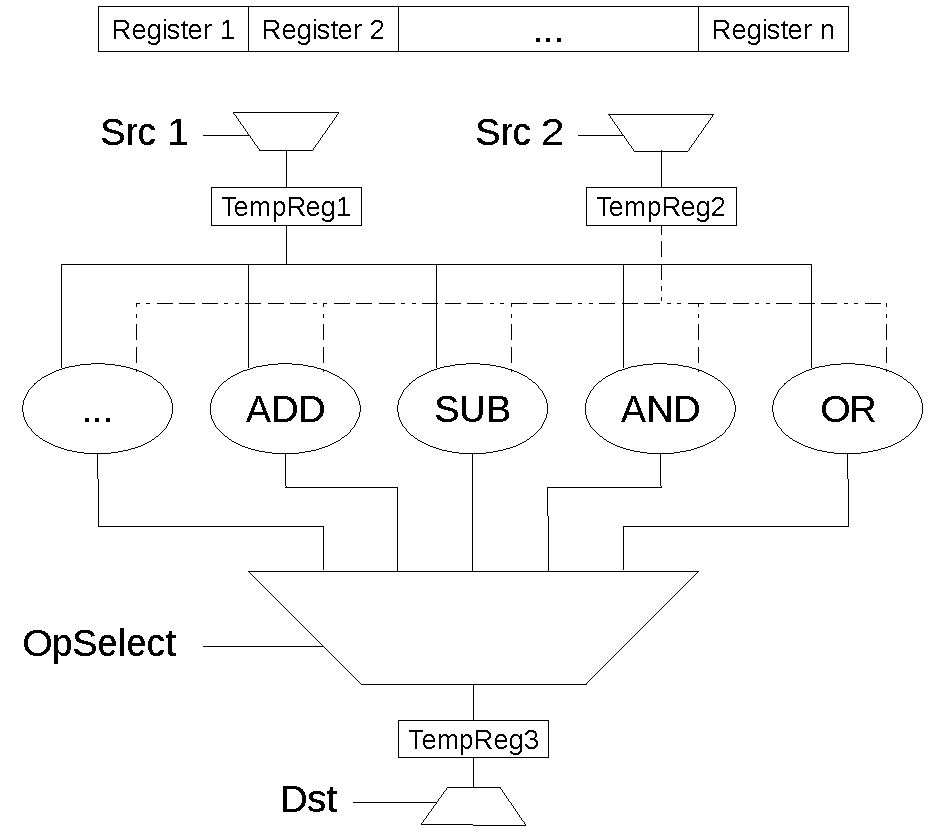
\includegraphics[width=5in]{IntroToAssembly/images/SimpleALUWithRegisters}
\label{fig:IntroToAssembly:SimpleALUWithRegisters}
\caption{A Simple ALU with registers. Note: I did not draw the lines from the Register File (the collection of Registers on top) to the muxes and also from the output back because it would have been too messy. I also changed the names of the inputs.}
\end{figure}

At this point, we have used our basic Digital Logic knowledge to build a CPU of sorts (at least the ALU part of one). We should also see that we now have four different inputs, the OpCode, the Src1, Src2 and then the Dst. We are now ready to talk about instruction encodings.

\subsection{Encoding Instructions in Binary}

For illustration purposes, let’s say that this computer that we are building will have 256 registers in the register file and will also include 256 different operations (we only show 4 above, but use your imagination). This distinction is very special because it is very neat. What this means is that we can encode all of the necessary information into a single 32-bit value. All we need to do is assign a particular OpCode value to each unique operation and then decide on an ordering of the 4 bytes.

To keep things consistent with the x86 ATT format (the one that GNU Assembler - GAS - uses) we will have the OpCode, followed by the SRC operands followed by the DST. So for example, if the ADD operation has OpCode number 5 and we are trying to add registers 1 and 15 together and store the sum into register 10 we might have the following: 

0x05 | 0x01 | 0x0F | 0x10

Knowing this information also means we can now decode any instruction. In particular, given the raw instruction bytes, we can take the first byte, look up into a table and then obtain the instruction being processed, the next two bytes will then be used to obtain the register numbers of the two source operands and finally the last byte will be used to obtain the register number for the output. The entire process of getting the instruction and decoding it is known as disassembly. In effect, disassembly takes the machine level input (the raw bytes) and transforms it into human readable input (assembly).

\subsection{Supporting Constants in Instructions}

At this point we have the ability to instruct the ALU to perform basic operations on registers. One might then ask, how does one load information into the registers in the first place? Some of you might think that it should be possible to load a constant value (a literal) into the registers such as loading the value 0 into a register, others might think of loading some data from memory into the registers, but then we haven't discussed memory yet, and finally someone else might suggest that all registers are loaded with default values such as a default of 0 and then it is up to the user to use the available instructions to calculate other values as needed. 

To the last point, imagine if there is an instruction operation \inlinedcode{INC} for "Increment", \inlinedcode{MOV} for "Move or copy", \inlinedcode{SHIFTLEFT} for "Shifting the first operand to the left the right operand number of times", and all registers are initialized to zero. If we want to load the value 17 (0x11) into the register R0 we will be able to do it using the following sequence of instructions.

\begin{code}
INC R0, X, R0 # We use X to represent a Don't Care in this case since INC only requires a single operand. R0 is now 1
MOV R0, X, R1 # Copy 1 into R1
INC R1, X, R1 # R1 is now 2
SHIFTLEFT R1, R0, R1 # R1 is now 4 since 2 (10b) << 1 is the same as (100b) which is 4
SHIFTLEFT R0, R1, R0 # R0 is now 1 << 4 or 10000b which is the same as 0x10
INC R0, X, R0 # Finally R0 is now 17
\end{code}

The previous example is also good for illustrating how assembly programming is just like any other programming. We are given a list of possible operations to make and it is up to us to figure out how we can make use of the limited set of operations to make something more complicated. 

This process is not that different from how we were able to use the basic components from digital logic to make the ALU in the first place. This is the general case for computing. Everytime we create something new, we create a new "abstraction" layer. Digital Logic created an abstraction layer that abstracted away the details of the transistors from the logic gate users, then the ALU has abstracted away the details of the logic gates (both discrete and sequential) to make friendlier and more familiar functions such as the \inlinedcode{ADD}, \inlinedcode{SUB}, etc. operations. We will do this until we get an assembly language, but it is easy or at least should be easy to imagine how this can continue until you get to higher order languages. 

Back to the point of discussion. We have thus far shown that we can use the available instructions to help initialize certain values into registers. What about loading these constant values into the registers in the first place?

\subsubsection{Loading Constants Directly}

Loading constant values into the registers will require some overloading of the instruction format that was discussed previously. Previously we have determined that the first byte of the instruction will be used to store the OpCode or the number of the operation to process. The other bytes will then be used to store the appropriate register numbers. In the previous example we also demonstrated and stated that sometimes there might be don't cares because certain operations do not require more than one operand. 

To introduce support for loading constants, we will now have to make decisions based on the OpCodes themselves. This can be easily supported as long as we have a quick way to identify all of the constant based OpCodes (let's say the first most significant bit of such OpCodes are 1b). In this case we will have 128 OpCodes that will deal with with register based operands and another 128 that deals with Constants. 

Since it doesn't make sense for the output to go into a constant, this also means that of the 4 bytes available in our 32-bit instruction format, only two are already taken. The first byte will contain the operation number (OpCode) to process and the last byte will be used to hold the destination register.

This leaves us with 2 bytes of space left to store the constant. So for example, imagine if we have an OpCode 0x80 (1000 0000b) for the \inlinedcode{MOV_C C, DST} instruction that moves a constant C into the register DST. Everything looks good and we now have the ability to support loading and using constant values in our operations.

\subsubsection{Supporting >2 byte Constants and Variable Length Instructions}

The problem that you might have noticed is that the Registers themselves are 4 bytes long but the constant is only 2 bytes. What do we do? 

On the one hand we can use the ALU trick above and just say that if you want to move a 4 byte constant (0x12345678) into a register then you will do something like the following

\begin{code}
MOV_C 0x1234, R0 # R0 = 0x1234
MOV_C 0x0010, R1 # R1 = 16
SHIFTLEFT R0, R1, R0 # R0 = 0x12340000
MOV_C 0x5678, R1 # R1 = 0x5678
OR R0, R1, R0 # R0 = 0x12345678
\end{code}

An alternative approach is to introduce variable length instructions. That is the length of the instruction (in bytes) is determined by which OpCode is being used. Constant-based operations might have different variants depending on the size of the constant. Two byte constants will result in 4-byte instructions (as we have discussed) and four byte constants will then result in 6 byte instructions. This design requires additional facilities and internal logic to dynamically determine how big the instruction is, but it is certainly possible.

In fact, the prior design is what ARM uses -- ARM uses 32-bit or 4-byte instructions -- and the latter is what x86 uses -- x86 uses variable length instructions ranging from 1-byte to 15-bytes. 

\subsection{Supporting Memory Operations in Instructions}
We are now left with the last solution to the original problem of loading initial values into the registers. How do we support the loading of values and constants from memory?

As you can probably guess by now, loading new values from memory will also require support for additional OpCode based logic where we further separate the OpCodes into ones that deal with registers only, ones that deal with constants and registers as well as ones that deal with memory and registers. Also with our recent discussion, you might wonder what happens if we have a lot of memory (let’s say 32-bit addressable or 4GB of addressable memory?). If the 4-byte instructions are not big enough to hold 4-byte constants how in the world will it be suitable or sufficient for addressing the entirety of memory?

This problem can be solved using the variable length instruction format as discussed previously, but it can also be done using some other tricks. The first technique is to use register-offset-based addressing. For example, we can create a new instruction for \inlinedcode{MOV_RO BASE, C, DST} where we will load the 4 bytes of contents from memory location BASE + C into DST. For example, we can continue with the 0x12345678 example above and load the contents of memory location 0x12345600 into register R1 using

\begin{code}
MOV_RO R0, -0x78, R1 # -0x78 still works since it fits within one byte in 2's complement
\end{code}
 
Similarly we can move the contents of 0x12345700 into register R2 using

\begin{code}
MOV_RO R0, 0x88, R2
\end{code}

While this works, there is always the limitation that we can only reference -128 to 127 of the address contained within a register. We can always work around this limitation by adding the desired offset into the register in the first place and then just loading the contents of memory directly from the register such as the following

\begin{code}
# Assume that we have moved 0x10000000 into R0 as shown before
# Assume that we have also moved 0x12345678 into R1 as before
ADD R0, R1, R2 # R2 = 0x22345678
MOV_RO R2, 0x0, R2 # R2 is now the contents of the memory location with address 0x22345678
\end{code}

Once again, other solutions are possible. It all depends on our imagination and the ability to use the basic operations given to build more and more advanced functionality.

At this point, we were able to use the basic discrete and sequential logic components to build an ALU that contains the most basic operations that includes variants to support using constants, accessing memory as well as just operating with registers. One question that might have nagged you and perhaps continues to do so is where do we get all of the instructions from in the first place?

\section{Storing the Instruction Stream}

The examples above showed sequences of instructions to perform interesting and more advanced operations, but where does one store all of those instructions?

First let’s remember that the instructions are just sequences of bytes. The raw bytes become instructions when the ALU processes them into their corresponding parts and interprets them accordingly. Recall how we first started with a 32-bit instruction format where each byte has a specific meaning. What this means is that given any 4-bytes, the ALU will treat the first one as an OpCode, the last byte as the destination register and then finally the two middle bytes depending on what the operation specified by the OpCode is. It will interpret it this way as long as you give it 4 bytes. 

Note in the case of variable length instruction formats such as x86, the actual number of bytes used will vary. While this is true, the fundamental observation that the ALU will interpret any bytes given to it as part of the instruction stream still holds.

This is the first major observation that warrants additional emphasis - as long as the ALU gets the bytes, the bytes will be treated as instructions. It doesn’t matter where the raw bytes come from. So where can we get them from?

\subsection{Storing Instructions in Infinite Instruction Registers}

In the simplest case we might imagine a completely separate set of registers RI being used to store the instructions. Let’s take this special theoretical case as an example and build from it.

To see how this works, we will just have to imagine that for the mini code samples we discussed above, each one of the instructions will be loaded into a sequence of registers RI0, RI1, RI2, … All that is left is for the ALU to start processing the first instruction at RI0, followed by the second and then the third until all of the instructions have completed. If you are wondering how we can known when all of the instructions have been processed, you can just imagine a special OpCode that is reserved to signify the END for example. 

This simple design works well as long as we have fixed length instructions. What happens when we have variable length instructions though? For example what should the size of each instruction register be for a similar x86 machine? Should it be 1 byte long or 4 bytes or perhaps 15 bytes and just forst each instruction, even 1 byte instructions, to be stored in its own 15-byte register? 

This dilemma brings makes the next design choice a bit obvious, but so does the realization that infinite register machines are not very realistic. It is much more realistic to have the instruction bytes be loaded into memory and have the ALU load each and every single instruction from memory instead. 

\subsection{Storing Instructions in Memory}

For illustration purposes let’s fist imagine that we have an infinite number of registers each of 1 byte in length. We didn’t like the 15-byte register design because many bytes will remain unused. In this design, we can no longer rely on each individual register containing its own instruction. Instructions can span across multiple registers. How do we keep track of things now?

As with many other things in Computer Science, we can keep track of which bytes we are interpreting as the current instruction by using another layer of indirection. We can simply introduce a special register called the Program Counter (also known as Instruction Pointer) that contains the register number of the current instruction (x86 uses this design) or the next instruction (ARM uses this design) -- the only real difference is when we update the counter either after the instruction is executed or before the instruction is executed. 

So tying this together with the previous examples, we now have a new register PC that will start with the value 0. In the 32-byte instruction design where each register contains another instruction, the PC register is incremented automatically every time an instruction is executed. This means that the PC will go through values of 0, 1, 2, 3, … corresponding with the R0, R1, R2, R3 we discussed previously.

In the case where each instruction can be of a different size and the registers are a single byte each, we will be adding the size of the current instruction to the PC instead of simply incrementing it each time. So for example, if the instructions that we will be executing are of size 4, 7, 8, 3, 2 respectively, the PC will go through values of 0, 4, 11, 19, 22, 24 respectively to signify that the ALU should process the instruction starting at R0, which the ALU recognizes is a 4 byte instruction that is stored in R0, R1, R2 and R3. The next instruction should therefore be in R4, which the ALU recognizes is a 7 byte instruction and so on.

At this point, we should make a very interesting observation. In this case where variable instruction lengths are used, if we somehow had an error where we started with PC having the value 1 instead of 0, then the instruction stream can be completely different because the actual operation as well as instruction length is determined by the ALU when the raw bytes are loaded from the registers. 

We can use x86 to illustrate a very quick example.
\begin{code}
seed@ubuntu:~/Desktop/SAMPLE$ echo -e -n "\xa1\x55\x89\xe5\x00" > TEST
seed@ubuntu:~/Desktop/SAMPLE$ objdump -m i386 -b binary -D TEST

TEST:     file format binary


Disassembly of section .data:

00000000 <.data>:
   0:	a1 55 89 e5 00       	mov    0xe58955,%eax

seed@ubuntu:~/Desktop/SAMPLE$ objdump -m i386 -b binary --start-address=0x1 -D TEST

TEST:     file format binary


Disassembly of section .data:

00000001 <.data+0x1>:
   1:	55                   	push   %ebp
   2:	89 e5                	mov    %esp,%ebp
	...
seed@ubuntu:~/Desktop/SAMPLE$ 

\end{code}

The first command in the sample above is used to write some raw byte values into a file named TEST. The second command uses the objdump program to disassemble the raw bytes. As we can see, the instruction that has been disassembled is a \inlinedcode{MOV} instruction. The constant value we are moving into the EAX register should look familiar. The third command uses objdump to disassemble again, however with an offset of 1 instead. The alternative stream is obvious.

Interestingly enough, if you think about the case of the 32-bit instructions (or cases where all instructions are of the same size), this problem doesn’t exist because the instruction boundaries are always clear and well defined. This means that an architecture such as ARM doesn’t have the multiple-instruction stream problem we just illustrated above (this isn’t fully true since ARM has different operating modes such as THUMB which uses 16 bit instructions instead of 32 so the problem can still exist, but not as bad as in x86). 
 
At this point, we should see how the introduction of a PC register can help keep track of where we are in terms of which raw bytes should be used for executing the current instruction. We should also see that the infinite single-byte instruction register design mentioned previously is not that different from the memory design that uses byte-addressing. Instead of storing the register number of the first byte of the current instruction, the PC will store the memory-address of the first byte of the current instruction.

\section{Chaining Instructions Using Control Flow Redirection}

At this point of our discussion, we have described how the basic elements from digital logic can be used to build an ALU which can support variable length instructions. However, there is the limitation that the instructions must be sequential - one after another. We haven’t discussed any means to change the control flow (flow of execution) yet. Importantly, we haven’t discussed any ways to perform loops, which would be nice if we wanted to implement that multiplier.

\subsection{Loops}

The simplest loop that we can define is perhaps a loop with a known number of iterations. These kinds of loops are simple, because we can simply “unroll” them which is to simply copy the loop body and paste it the number of iterations turning it into a single stream of instructions.

The next simplest loop is the infinite loop where we execute the body of the loop an infinite number of times, meaning there is no way to fully unroll the loop or even come up with an upper bound and unroll the loop using that as an iteration. The infinite loop is simple because all we need is a way to tell the ALU that the next instruction to execute is actually at the beginning of the loop once we have reached the end of the body. 

Given our discussion about using a PC to keep track of where we are, what we are missing is a simple instruction/operation that can write a value to the PC. Once again, there might be different variants that writes an offset to the PC (using the current value as the base) or a constant value or even reading the value from a register or memory just like all of the variants we discussed previously. These types of instructions are normally called “branches” (ARM parlance) or “jumps” (x86 parlance) and they are effectively the same as a \inlinedcode{MOV} operation where the destination register is PC instead of a normal register number.

For example, if we have 32 bit instructions from the early examples, the following sample assembly code will give us an infinite loop that increments the register R0 forever.

\begin{code}
INC R0, X, R0 # Assume that this instruction is stored in register RI0 or memory location 0
MOV 0, X, PC # we can use something like JMP 0 as a shortcut macro where PC as the destination register is implied.
\end{code}

\subsection{Conditional Control Flow Transfers}

After infinite loops, the next easiest (or actually the only remaining category in our discussions) is the variable iteration loop, where the loop ends when a condition is satisfied -- think of a “while” loop. So how do we check conditions? 

In effect, we need a conditional branch or a conditional jump. Perhaps the simplest thing we can imagine is something such as “jump if register is not 0” which we can call \inlinedcode{JNZ} for short. For example, if I want to count register R0 from 10 down to 0, we can do something as follows (to make things a little bit more interesting let’s assume all instructions are 32-bits long and the PC contains the memory address of the current instruction to execute and these instructions start at memory address 0x12345678):

\begin{code}
MOV_C 0xA, R0 # R0 = 10
MOV PC, X, R2 # R2 = PC = 0x1234567C, save the address
SUB_C R0, 0x1, R0 # R0 = R0 - 1
JNZ R0, X, R2 # if R0 == 0 then first byte of next instruction is located at memory address in R2, meaning we will go back to the MOV PC, X, R2 instruction
\end{code}

Alternatively, if there was a \inlinedcode{JNZ} instruction that takes an “offset” from the current PC value then the loop can be written as

\begin{code}
MOV_C 0xA, R0 # R0 = 10
SUB_C R0, 0x1, R0 # R0 = R0 - 1
JNZ_C R0, -0x4 # if R0 == 0 then first byte of next instruction is 4 bytes before current instruction, since currently PC is at 0x12345680, we will execute the instruction at 0x1234567C next, which is the SUB\_C R0, 0x1, R0 instruction. Notice how this loop is a bit tighter and more efficient than the previous one since the MOV PC instruction from the loop before is unnecessary. We certainly could have fixed it by adding an offset of 8 bytes into R2 right before the SUB\_C instruction (I’ll leave it up to you to figure that out).
\end{code}

You can certainly think of other ways to do this as well.

\subsubsection{Direct Versus Indirect Jumps}

Now I want to point out something very interesting about the two cases above. The first case is known as an “indirect jump” or an “indirect branch” because the target address (the value to store into PC) is itself stored in another location -- a register in this example, but it’s also an indirect jump if it’s stored in memory. The second case is a direct jump because the target address is always known. 

To be more precise, while the value of the target address does depend on the PC register, and the value of the PC register might not be known exactly until runtime, but given that we know the value has to be where the \inlinedcode{JNZ_C} instruction is, the next instruction is guaranteed to be the \inlinedcode{SUB_C} instruction unless the raw bytes representing the instructions themselves have changed in memory. 

That is, if the value of PC has changed by the time we execute \inlinedcode{JNZ_C}, the new value of PC - 0x4 is still where \inlinedcode{SUB_C} is. This is not true for the first case since if R2 changed values by the time we execute the JNZ instruction (you might not fully see why this is the case until we talk about functions, things will be more clear then), the next instruction will start at whatever the new value is. 

\subsubsection{Direct and Indirect Memory Addressing}
Note that memory accesses can also be direct and indirect. The examples above have only used indirect addressing given that \inlinedcode{MOV_RO} is a constant offset from a particular register. As discussed previously though, it is also possible to use constant memory addresses if we have long enough instructions as in variable length instruction sets. 

Notice that we said that PC based offsets can also be considered direct addressing as long as the instruction stream (the memory containing instructions) does not change. In general, the way we reason about direct versus indirect addressing is by asking whether the target address can be determined statically (direct) versus dynamically (indirect).

In other words, direct addresses are ones that can be determined without running the program (statically) or that any execution of the program will result in the same address while indirect addressing uses memory addresses that can change through different executions of the program and we can only be sure of the value at runtime (dynamically). To see how this might work, let’s assume that there is another special register called \inlinedcode{PC_BASE} which will always contain the base memory address of the first instruction in the instruction stream. 

Since we have thus far assumed that instructions start at memory address 0, this would mean that \inlinedcode{PC_BASE} is set to 0. Thus, any offsets from \inlinedcode{PC_BASE} will be 0 + offset. This also means that we can move the instructions to any part of memory and just set \inlinedcode{PC_BASE} accordingly when the program starts. Notice that all of these offsets, while technically are calculated relative to the value of a register (\inlinedcode{PC_BASE}), since the value of \inlinedcode{PC_BASE} doesn’t change throughout any execution of the program, these offset addresses are still direct. A quick extension of this idea will show that PC based offsets are also direct.

\subsubsection{More Conditionals}

We now have a way to support things like loops by introducing conditional jumps (which are basically \inlinedcode{MOV}s but with the destination being the PC register and where the update only works if a register does not contain the value 0). If you are wondering what about conditions such as ZERO or GREATER THAN, then I want you to convince yourself that you can support these by creating meta instructions using the other ALU operations. For example, ZERO can be supported as \inlinedcode{JNZ_C +0x8} followed by the \inlinedcode{JMP} instruction.  The \inlinedcode{JNZ_C +0x8} will ensure that if it is not zero, we will skip the next instruction and if it is zero we will process the next instruction which happens to be a JMP to the intended target. Once again, what you can do is left up to your imagination.

We have also introduced two potential problems with having the ability to write to the PC. First, we have indirect jumps where what we are writing to the program counter might not be known until you start executing the instruction stream. This also means that anyone who controls the contents of the source register or memory will also control what instructions will be executed next. The second thing we learned (really first in terms of when we introduced it) is that in the case of variable length instructions, we can have alternative instruction streams that could prove problematic. 

As a quick side note, CPUs normally include a special Flags Register where each bit represents a specific condition and is updated after each and every single operation is executed - e.g. one bit is used to signal whether the previous operation resulted in a 0 (Zero Flag) and another is used to signal whether the previous operation resulted in a negative value (Sign Flag). In this way, the conditional jumps can then be based on the condition (or status) of specific bits in the Flags Register. 

Now that we know how to support loops (and naturally conditional processing - if statements - in general) you might be wondering about functions, which is a very nice way to organize code. This will be the last topic of discussion in this introduction to assembly.

\subsection{Functions}

In reality, as long as you understand the ability to perform jumps or branches then you should understand functions. Functions is just an added layer of abstraction on top of jumps by introducing meta instructions that save the current value of the PC so it can be restored later. Just like the PC, we can support this by introducing another register that we can call RR for the Return Register (ARM calls it the link register and x86 doesn’t have such a thing).

Once we introduce this new register, the difference between a function call and a normal jump is that when we “call” a function, we expect to continue execution at the next instruction after the function we called “returns”. This is achieved by automatically storing the value of the next instruction in the RR register prior to transferring control to the function being called.

Let’s consider the following sample assembly based on the example above where the instructions start at address 0x12345678. This time, I prepended each instruction with it’s memory address for easier understanding.

\begin{code}
0x12345678:	JMP 0x1234568C
0x1234567C:	MOV_C 0xA, R0 # R0 = 10
0x12345680:	SUB_C R0, 0xA, R0 # R0 = R0 - 1
0x12345684:	JNZ_C R1, -0x4 # if R1 == 0 then first byte of next instruction is 8 bytes before current instruction
0x12345688:	MOV RR, X, PC # PC = RR
0x1234568C:	ADD_C PC, 0x8, RR # RR = PC + 0x8 = 0x12345694
0x12345690:	JMP_C -0x14 # PC = PC - 0x14 = 0x1234567C
0x12345694:	END
\end{code}

As you can see, the first thing this little assembly code snippet does is to jump to 0x1234568C. From there the value of RR is updated to where the END instruction would be followed by a offset based jump to 0x1234567C. The instructions will execute in a loop decrementing R0 from 10 until R0 is 0. At this point, the JNZ instruction at 0x12345684 won’t be taken and the next instruction executed which restores PC to the saved address of 0x12345694 which means the next instruction is \inlinedcode{END}.

Now I wrote the previous example in the way I did to illustrate that the boundaries of a “function” can be seen in between addresses 0x1234567C and 0x12345688 (inclusive). Additionally, we can also consider creating a new meta-instruction using the instructions at 0x1234568C and 0x12345690. This new instruction can be the CALL instruction where we can “CALL” the function starting at offset -0x14 which is the function at 0x1234567C. Similarly, the instruction at 0x12345688 can be called the \inlinedcode{RET} instruction since it restores the value in the Return Register (RR) back into the PC. 

This illustration is important to show that once again, we can build more and more complex functionality using the basic operations we defined for the ALU initially. This should also give you a sense of why understanding the fundamentals of how these things work might help you better understand the exercises in the last couple of assignments.

The final thing that you might have observed is that using the RR might give us the ability to store a return address, but it is limited to having function calls being one deep. Meaning if we have a function f() that calls g(), g() cannot call another function and furthermore no other function could have called f(). 
1.5.4  Nested Function Calls
As you would likely guess, we can solve this problem by introducing another register file for storing the return addresses as well as another special register (let’s call it RC) to keeping track of where the current Return Register value is. In this way, we will have three separate register files, the infinite registers for data, the infinite registers for instructions and the infinite registers for control data (e.g., return addresses). 

Just like how the \inlinedcode{JMP} instruction is then a special case of the \inlinedcode{MOV} instruction that uses the PC as the implied destination operation, we can introduce new instructions such as CALL that not only stores the value of the next instruction into RR and then moves the target into the PC register as discussed previously, but now \inlinedcode{CALL} will actually first increment RC so it will refer to the next available register in the Return Registers register file, and then stores the value of the natural next instruction into that return register followed by the \inlinedcode{JMP}. 

Similarly, \inlinedcode{RET} will not only load the value of the current Return Register (specified by RC) into the program counter PC, but it will also automatically decrement RC (notice how this increment and decrement behavior of mimics that of a stack - this is expected).

As a quick note, this design where the control data (Return Registers) and regular data (Registers) are separated from each other is known as a Harvard Architecture. A Von-Neumann Architecture is one where there the two aren’t separated. This makes a bit more sense when we consider how wasteful it might be to create a completely separate register file just for storing return addresses when we don’t even know how deep function calls can be. 

\section{Mapping Register Files into Memory}

At any rate, similar to how we took the infinite single-byte instruction registers and mapped it into memory, we can do the same with the return registers. In fact, if we think about the entirety of memory (let’s say 4GB of it) we might want to segment the memory into 4 equal sized chucks where the first GB is used for instructions, second GB for regular data, third GB for return addresses and finally the last GB for special things such as privileged access to devices or the kernel. We will expand on this when we discuss segmentation.

Furthermore, the observation that the increment and decrement behavior of the RC makes the series of Return Registers seem like a stack should give us enough motivation to implement or introduce additional instructions such as \inlinedcode{PUSH} and \inlinedcode{POP} that will treat a portion of memory (e.g., the third GB mentioned above) as a stack. 

The only question that remains is whether the stack grows up from low memory to high or grows down from high memory to low. In either case, we will need to introduce yet another special register to keep track of where the top of the stack is (both ARM and x86 calls it the Stack Pointer register). In the case of stacks growing up towards high memory PUSH will add the number of byte pushed to the stack pointer register and subtract from it if the stack grows down. While the details are different, the fundamental idea of a segment of memory behave like a stack is the same. 

Finally, as a quick note, the idea of dedicating a section of memory to behave like a stack is basic. While we got to this point by saying that the chain of function calls can be naturally represented as a stack, it doesn’t mean that the stack can only be used to store return addresses. In fact, modern systems normally like to use the stack to store both return addresses as well as data that is local to the current instantiation of a function being called. We call the boundaries between the different function instantiations “frames.” 

\section{Conclusion}
We will end this introduction to assembly here. More details on how this applies to x86 can be found in the assignment notes. 

All in all, we have effectively built up from basic digital logic elements up to a fairly sophisticated processor by introducing more and more complex abstraction layers. Each layer introduced new operations which we have shown to be built up of a combination of operations found in the underlying abstraction layers. 

We have also shown that by introducing more and more specialized registers and indirection, we have opened up more and more opportunities for errors to occur since these specialized registers can also be written to (the registers or memory that the value is loaded from can also be written to) leading to difficulties in predicting what the values could or should be (think Control Flow Integrity) and in the case of variable length instructions perhaps even completely different and unexpected instruction streams.

